\documentclass[12pt]{article}
\usepackage[utf8]{inputenc}
\usepackage{float}
\usepackage[fleqn]{amsmath}
\usepackage{mathtools}
\usepackage{bigints}
\usepackage{tikz}
\usepackage{pgfplots}
\pgfplotsset{compat=newest}
\usepgfplotslibrary{fillbetween}
\usepackage[hmargin=3cm,vmargin=6.0cm]{geometry}
\topmargin=-2cm
\addtolength{\textheight}{6.5cm}
\addtolength{\textwidth}{2.0cm}
\setlength{\oddsidemargin}{0.0cm}
\setlength{\evensidemargin}{0.0cm}
\usepackage{indentfirst}
\usepackage{amsfonts}

\begin{document}

\section*{Student Information}

Name : Emre Geçit

ID : 2521581


\section*{Answer 1}

\paragraph{a)}

$X$ and $Y$ are independent iff$f(x)f(y) = f(x,y)$.\\\\
This function has a nonzero value inside\\\\
$-\sqrt[]{1-x^2} < y < \sqrt{1-x^2}$\\\\
$-\sqrt{1-y^2} < x < \sqrt{1-y^2}$.\\\\

Since integral of $f(x, y)$ outside these boundaries is zero, integrating between these boundaries will be enough.\\\\
$f(y) = \bigint_{-\sqrt{1-x^2}}^{\sqrt{1-x^2}}  1/\pi\,dx$\\\\
$f(y) = \frac{2\sqrt{1-x^2}}{\pi}$\\\\
$f(x) = \bigint_{-\sqrt{1-y^2}}^{\sqrt{1-y^2}}  1/\pi\,dy$\\\\
$f(x) = \frac{2\sqrt{1-y^2}}{\pi}$\\\\
$f(x)f(y) = \frac{2\sqrt{1-y^2}}{\pi} \frac{2\sqrt{1-x^2}}{\pi} = \frac{4\sqrt{(1-x^2)(1-y^2)}}{\pi^2}$\\\\
$f(x)f(y) \neq f(x,y)$\\\\
Since $f(x)f(y)$ is not equal to $f(x,y)$, random variables X and Y are not independent.
\paragraph{b)}
From a, marginal pdf for $X$ is $f(x) = \frac{2\sqrt{1-x^2}}{\pi}$ and marginal pdf for $Y$ is $f(y) = \frac{2\sqrt{1-y^2}}{\pi}$\\\\
\paragraph{c)}
Expected value for $f(x)$ is $E(X) = \bigint_{-1}^{1} xf(x) \,dx = \bigint_{-1}^{1} \frac{2x\sqrt{1-x^2}}{\pi} \,dx$\\\\
Solving this integral we find $E(X) = \frac{-2 (1 - x^2)^{3/2}}{3 \pi} \vert_{-1}^{1} = 0$\\\\
\paragraph{d)}
$Var(X) = E(X^2) - \mu ^2$\\\\
$E(X^2) = \int_{-1}^{1} x^2 f(x) \,dx = \int_{-1}^{1} \frac{2x^2\sqrt{1-x^2}}{\pi} \,dx = 0.25$\\\\
$\mu = E(X) = 0$ (from part c)\\\\
$Var(X) = 0.25 - 0^2 = 0.25$
\newpage
\section*{Answer 2}
\paragraph{a)}
Since these two events are independent $f(t_A, t_B) = f(t_A)f(t_B)$\\\\
$f(t_A) = 1/100$ and $f(t_B) = 1/100$\\\\
$f(t_A, t_B) = 1/100 \times 1/100 = 1/10000$\\\\
\paragraph{b)}
$P(t_A < 10, t_B > 90) = P(t_A < 10)P(t_B > 90) = \int_0^{10}f(t_A)\,dt \times \int_{90}^{100}f(t_B) \,dt$\\\\
$=(\frac{t}{100}\vert_0^{10})\times(\frac{t}{100}\vert_{90}^{100}) = 0.1 \times 0.1 = 0.01$\\\\
\paragraph{c)}
$P(t_A < t_B + 20)$\\\\
This probability distribution can be shown with a 2d graph as follows:\\\\

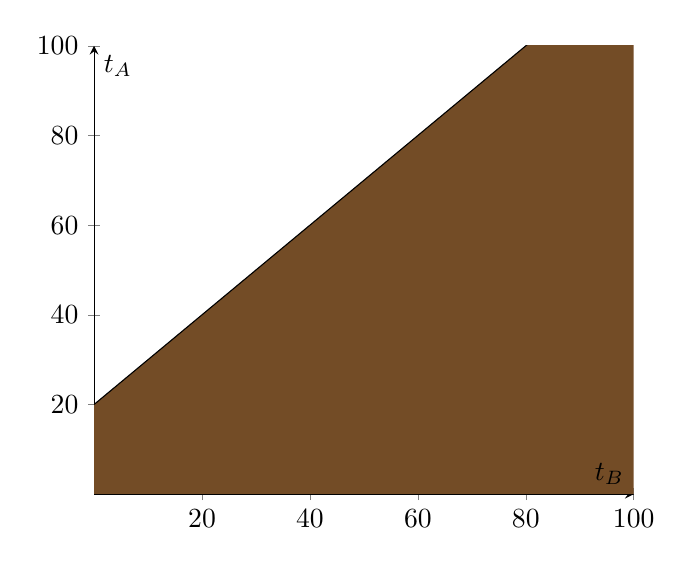
\begin{tikzpicture}
    \begin{axis}[
        axis lines = middle,
        xlabel={$t_B$},
        ylabel={$t_A$},
        xmin = 0,
        xmax = 100,
        ymin = 0,
        ymax = 100]
        \addplot [name path = X, domain = 0:100] {0};
        \addplot [name path = A, domain = 0:100] {x+20};
        \addplot fill between [of = A and X];
    \end{axis}
\end{tikzpicture}

The probability $P(t_A < t_B + 20)$ is the ratio between the area under the curve $t_A < t_B + 20$ to the probability space.\\\\
That is $6800/10000 = 0.68$\\\\
\newpage
\paragraph{d)}
Likewise the previous question, this probability can also be modelled as a 2d graph.\\\\
$P(|t_A - t_B| < 30):$\\\\
$|t_A - t_B| < 30 \equiv (t_B - 30 < t_A < t_B + 30)$\\\\
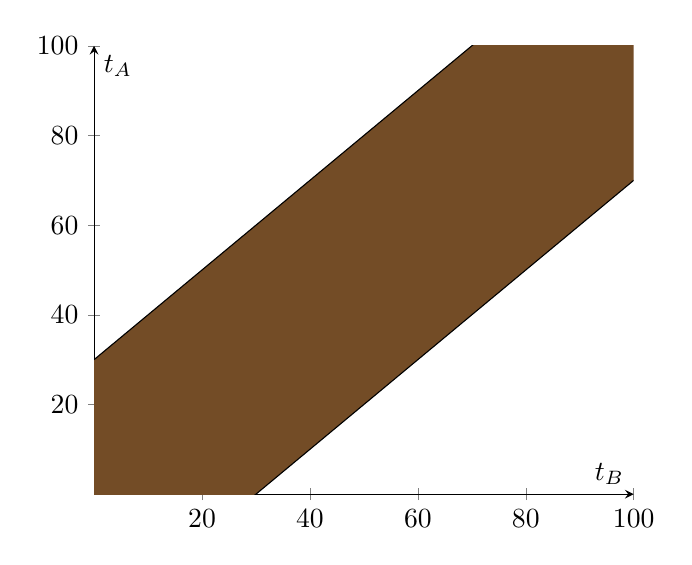
\begin{tikzpicture}
    \begin{axis}[
        axis lines = middle,
        xlabel={$t_B$},
        ylabel={$t_A$},
        xmin = 0,
        xmax = 100,
        ymin = 0,
        ymax = 100]
        \addplot [name path = B, domain = 0:100] {x+30};
        \addplot [name path = A, domain = 0:100] {x-30};
        \addplot fill between [of = A and B];
    \end{axis}
\end{tikzpicture}

$P(|t_A - t_B| < 30) = 5100/10000 = 0.51$\\\\

\section*{Answer 3}
\paragraph{a)}
Let $F_T$  be the cdf of the random variable $T$.\\\\
\begin{flalign*}
    F_T(t) & = P(T < t)\\
           & = 1 - P(T \geq t)\\
           & = 1 - P(min\{X_1, X_2, ..., X_n\} \geq t)\\
           & = 1 - P(X_1 \geq t, X_2 \geq t, ..., X_N \geq t)\\
           & = 1 - P(X_1 \geq t)P(X_2 \geq t)...P(X_N \geq t)\\
           & = 1 - e^{-t\lambda_1-t\lambda_2-...-t\lambda_N}\\
           & = 1 - e^{-\sum_{n = 1}^{N}t\lambda_n}\\
\end{flalign*}
\newpage
\paragraph{b)}
Let $T$ be the first moment that any of the computers fails and $X_n$ be the random variable that represents the time that computer $n$ fails.\\\\
$T = min\{X_1, X_2, ..., X_n\}$\\\\
Using the formula from part a, we get $F_T(t) = 1 - e^{-\sum_{n = 1}^{N}t\lambda_n}$\\\\
$\lambda_n = n/10$\\\\
We get, $F_T(t) = 1 - e^{-\sum_{n = 1}^{N}\frac{nt}{10}} = 1 - e^{-55/10}$\\\\
This cdf in the form of a exponential cdf. Then $\lambda = -(-55/10) = 55/10$\\\\
$E(T) = 1/\lambda = 10/55 = 0.18$\\\\

\section*{Answer 4}
\paragraph{a)}
At least \%70 of the participants are undergraduate students means that there are at least 70 undergraduate students among the participants.\\\\
The number $U$ of undergraduate students has binomial distribution with $n = 100$ and $p = 0.7$, $\mu = 74$ and $\sigma = \sqrt{100*0.74*(1-0.74)} = 4.386$.\\\\
Applying the central limit theorem with the continuity correction,\\\\
$P(U \geq 70) = P(U > 69.5) = P(\frac{U-\mu}{\sigma} \geq \frac{69.5-\mu}{\sigma})$\\\\
$P(Z > \frac{69.5-74}{4.386})$\\\\
$P(Z > -1.03) = 1 - P(Z \leq -1.03)$\\\\
$P(Z \leq -1.03) = \Phi(-1.03) = 0.1515$\\\\
$P(Z > -1.03) = 1 - P(Z \leq -1.03) = 0.8485$\\\\
The probability that at least \%70 of participants are undergraduate students is $0.8485$\\\\

\newpage
\paragraph{b)}
At most \%5 of the participants are pursuing a doctoral degree means that there is at most 5 doctoral students among the participants.\\\\
The number $D$ of participants that are pursuing a doctoral degree has binomial distribution with $n = 100$ and $p = 0.1$, $\mu = 10$ and $\sigma = \sqrt{100*0.1*(1-0.1)} = 3$\\\\
Applying the central limit theorem with the continuity correction,\\\\
$P(D \leq 5) = P(D < 5.5) = P(\frac{D-\mu}{\sigma} \leq \frac{5.5-\mu}{\sigma})$\\\\
$P(Z \leq \frac{5.5-10}{3}) = \Phi(-1.5) = 0.0668$\\\\
The probability that at most \%5 of participants are pursuing a doctoral degree is $0.0668$\\\\

\end{document}

